
\textbf{مورد استفاده:}
ثبت‌نام
\\
\textbf{شرح مختصر :UC}
این قسمت مهمان در سایت ثبت‌نام می‌کند.
\\
\textbf{پيش شرط:}
 دانشجو باشد.
\\
\textbf{سناريو اصلی:}
\begin{enumerate}
\item
شروع
\item
مهمان دکمه ثبت‌نام را انتخاب می‌کند و سیستم فرم ثبت‌نام را به مهمان نمایش می‌دهد.
\item
مهمان فرم را تکمیل می‌کند و با دکمه ارسال، فرم تکمیل شده را به سیستم ارسال می‌کند.
\item
سیستم فرم ثبت‌نام را بررسی می‌کند و اطلاعات فرم را در بانک اطلاعات ثبت می‌کند.
\item
پایان
\end{enumerate}

\noindent
\textbf{پس شرط:}
ندارد.
\\
\textbf{سناريوهای فرعی:}
\\
\textbf{سناريو فرعی 1:}
خطا در اطلاعات وارد شده
\\
\textbf{شرح مختصر :UC}
این سناریو در مرحله ۴ سناریو اصلی در صورت خطا در اطلاعات وارد شده فرم ثبت‌نام اجرا می‌شود.
\begin{enumerate}
\item
شروع
\item
اطلاعات فرم بررسی می‌شود و خطاها مشخص می‌شوند.
\item
یک پیغام به مهمان نمایش داده می‌شود و درخواست اصلاح اطلاعات وارد شده را دارد.
\item
از مرحله 3 سناریو اصلی ادامه پیدا می‌کند.
\item
پایان
\end{enumerate}

\noindent
\textbf{سناريو فرعی 2:}
کاربر با موفقیت ایجاد شود.
\\
\textbf{شرح مختصر :UC}
این سناریو در مرحله ۴ سناریو اصلی در صورت موفقیت آمیز بودن ثبت‌نام اجرا می‌شود.
\begin{enumerate}
\item
شروع
\item
اطلاعات فرم بررسی می‌شود و یک پیغام به مهمان نمایش داده می‌شود که اطلاعات با موفقیت ثبت و کاربر ایجاد شده است.
\item
از مرحله 4 سناریو اصلی ادامه پیدا می‌کند.
\item
پایان
\end{enumerate}

\noindent
\textbf{سناريو فرعی 3:}
کاربر موجود باشد.
\\
\textbf{شرح مختصر :UC}
این سناریو در مرحله ۴ سناریو اصلی در صورت وجود کاربر در بانک اطلاعات اجرا می‌شود.
\begin{enumerate}
\item
شروع
\item
یک پیغام به مهمان نمایش داده می‌شود که اطلاعات کاربری از قبل وجود دارد و دکمه ورود به سایت نمایش داده می‌شود.
\item
پایان
\end{enumerate}

\noindent
\textbf{پس شرط:}
ندارد .


\begin{figure}[H]
	\centering
	\includegraphics[width=.7\textwidth]{Diagram/2.Activity/ثبت‌نام.png}
	\caption{دیاگرام فعالیت ثبت‌نام}
	\label{fig:a:ثبت‌نام}
\end{figure}
\begin{figure}[H]
\centering
\includegraphics[width=.7\textwidth]{Diagram/3.StateMachine/ثبت‌نام.png}
\caption{دیاگرام حالت ماشین ثبت‌نام}
\label{fig:sm:ثبت‌نام}
\end{figure}
\begin{figure}[H]
	\centering
	\includegraphics[width=1\textwidth]{Diagram/4.Collaboration/1.Sequence/ثبت‌نام.png}
	\caption{دیاگرام توالی ثبت‌نام}
	\label{fig:s:ثبت‌نام}
\end{figure}
\begin{figure}[H]
\centering
\includegraphics[width=1\textwidth]{Diagram/4.Collaboration/2.Communication/ثبت‌نام.png}
\caption{دیاگرام همکار ثبت‌نام}
\label{fig:c:ثبت‌نام}
\end{figure}
